\clearpage
\section{前向渲染与延迟着色}\label{sec:lighting-paths}

拱门上有一盏灯，面前是一根石柱。把砖纹读出来，只能知道石柱本身的颜色；要得到屏幕上那条明暗交界，还要知道表面朝向和灯的位置。在 OpenGL 主绘制里，石柱的每个可见片元读一次材质，随后在网格着色器中计算直接光、阴影和环境光，把结果写进 HDR 场景颜色图。这样的处理叫前向渲染\termenglish{forward shading}。即使提前画过一遍深度，实际给石柱算光的仍是这次网格绘制。

\figpanel{lighting-pipelines}{读每行中间的方框可以找到负责光照的着色器。箭头表示左边的结果供右边读取。第二行选用编辑器已有的 Clustered lights；第三行展示分簇灯表可用于前向渲染的位置。}

Vulkan Lit 选用光栅主表面时，把这件事拆成两次。\code{VulkanDraw::DrawSurfaces} 先画网格，留下可见面的底色、世界空间法线和深度。这组描述每个像素表面的图通常称为几何缓冲\termenglish{G-buffer}。程序用深度和相机矩阵还原表面位置，随后能在同一位置计算直接光、间接光和环境遮蔽。将光照留到表面选好以后再计算，称为延迟着色\termenglish{deferred shading}。LearnOpenGL 的例子用全屏四边形读这些图，Redflag 的光照路径用计算着色器逐像素处理。

选择 Clustered lights 时，第一道计算把可能照进各个空间格子的灯号写进表，第二道计算读表面和灯表，得到直接光图。把同一张灯表交给实际绘制石柱的片元着色器，就是图中第三条路径。Forward+ 描述的是这项分工，使用灯号表本身只说明做过光源筛选。

\readings{\refitem{https://learnopengl.com/Advanced-Lighting/Deferred-Shading}{LearnOpenGL · The G-buffer}\quad
\refitem{https://github.khronos.org/Vulkan-Site/samples/latest/samples/performance/subpasses/README.html}{Khronos · Deferred rendering}\quad
\refitem{https://doi.org/10.2312/conf/eg2012/short/005-008}{Harada 等 · Forward+，第 2 节}}

\clearpage
\section{灯表从计算传到片元}

在 $16\times16$ 像素的屏幕小块里，近处的玻璃和远处的石柱可能正好重叠。Redflag 再按观察深度将小块分成 16 段；每段都有自己的灯表。一组 32 盏灯共用一个无符号整数，最低位为 1 表示本组的第一盏灯有机会照进这一段。着色时只遍历置为 1 的那些位，再检查实际表面与灯的距离和朝向。已有的 49 灯 Sponza 对照里，每个可见像素平均留下 18.11 盏候选灯，逐像素 RGB 与 CPU 遍历全部灯的最大差约为 $1.2\times10^{-7}$。这两个数分别衡量筛选量和颜色误差。

\codewhere{现有着色代码}{Redflag/src/Redflag/Renderer/ScreenSpace/Shaders/ClusterShade.comp}{main}
\begin{lstlisting}
Surface s = surfaces[i];
(*@\rhicomment{// i 对应一个已画好的像素，按它的位置找到所属的灯簇。}@*)
uint start = clusterAt(uvec2(p) / tile,
                       depthSlice(depthOf(s.position.xyz))) * words();
\end{lstlisting}

接入分簇 Forward+ 时，\path{ClusterCull.comp} 可以继续建表。现有灯表由 \code{ScreenEffects} 持有，图形绘制的资源布局只列出材质贴图。绘制命令需要同时取得本视口的灯、掩码、相机和分簇设置。后端在同一队列上先记录建表，再设置从计算写入到片元读取的依赖。切视口时换到相应的灯表，直到该帧完成才可覆盖。

\codewhere{拟议片元伪代码 · 现有材质入口}{Redflag/src/Platform/Vulkan/Shaders/Mesh.frag}{main}
\begin{lstlisting}
surface = ReadMeshMaterial(fragment)
cell = ClusterAt(fragment.pixel, ViewDepth(surface.position))
(*@\rhicomment{// 这里给正在光栅化的表面算光，每片玻璃都有自己的位置。}@*)
for light in frame.lights[cell]:
    color += ShadePointLight(surface, light)
\end{lstlisting}

实现时可把两条路径共有的衰减和漫反射计算提取为一个着色器函数。需要 GTAO、SSR 和 TAA 时仍要给它们保留法线、深度或历史图。第一轮验收应固定灯半径、曝光和相机，让两条路径输出线性直接光，另给石柱前摆一片玻璃，检查片元按玻璃自己的深度选灯。若测成本，还要把建表、画网格以及这些效果所需的图都计入同一帧。

\readings{\refitem{https://www.cse.chalmers.se/~uffe/tiled_shading_siggraph_2012.pdf}{Olsson 等 · Tiled and Clustered Forward Shading，图 1}\quad
\refitem{https://www.gdcvault.com/play/1016519/Forward-Rendering-Pipeline-for-Modern}{GDC Europe · Forward Rendering Pipeline for Modern GPUs}}

\clearpage
\section{玻璃后面的背景颜色}

近处的柱子能挡住玻璃，玻璃又能把后方的网格纹向一侧推开。延迟着色保留了每个像素最近的不透明表面；为了看见两层玻璃，OpenGL 先画实心物体和天空，再调用 \code{Renderer3D::DrawTransparency}。它保存背景颜色和深度，把每片玻璃的颜色、法线和厚度按权重累加。最后一次全屏绘制才混合玻璃与背景。Vulkan Lit 也为透明面单独绘制，合成安排在体积雾之后、TAA 之前。

\begin{center}
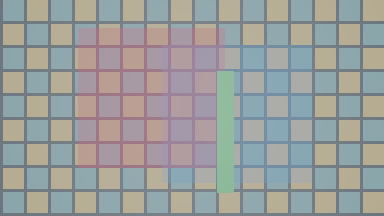
\includegraphics[width=.47\linewidth]{../../../output/profiling/gl-transparency/straight.png}\hfill
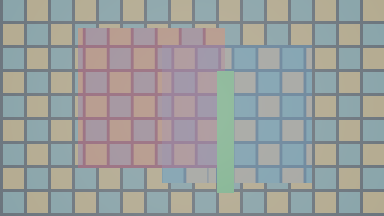
\includegraphics[width=.47\linewidth]{../../../output/profiling/gl-transparency/refracted.png}
\captionof{figure}{OpenGL 实测，每张 $384\times216$ 像素。两块玻璃前面有一根绿柱。左图折射率为 1；右图调到 1.52，厚度为 0.45 个场景单位。对照粉色玻璃的左边缘，背景竖线在右图中有横向位移，前景柱的位置与颜色保持一致。}
\end{center}

当折射位置落在两个像素之间时，会取周围四个背景像素按距离混合。若只看最近那个像素的深度，另外三个里仍可能有属于前景柱的颜色。测试只改变柱子的颜色，保持玻璃、墙和相机不动。旧取法在柱子外产生了最大 0.311768 的线性 RGB 通道差。按四个位置分别检查深度以后，柱外所有通道的差值降为零。测试扫描四个玻璃厚度，让采样点落到柱边缘的不同位置。

\codewhere{旧写法 · 实测复现}{RedflagForge/assets/shaders/Transparency_Composite.glsl}{合成入口 main}
\begin{lstlisting}
(*@\rhicomment{// 只检查一个深度，但下面的颜色采样会混合四个邻居。}@*)
if (texelFetch(u_OpaqueDepth, ivec2(uv * size), 0).r >= normalDepth.w)
    background = texture(u_Background, uv).rgb;
\end{lstlisting}
\codewhere{修正后的源码}{RedflagForge/assets/shaders/Transparency_Composite.glsl}{BackgroundAt}
\begin{lstlisting}
(*@\rhicomment{// 坐标 tap 对应前景时，这一份改取玻璃正后方的原色。}@*)
vec3 color = texelFetch(u_OpaqueDepth, tap, 0).r < glassDepth
    ? original : texelFetch(u_Background, tap, 0).rgb;
\end{lstlisting}

RenderDoc 回放中，事件 10 和 17 画出实心物体；54、62 分别累加两片玻璃；75 只向主画面的颜色图写入。换两片玻璃的提交顺序，全部像素的 RGB 完全一致。屏幕外的背景仍需用原图近似，而两层玻璃的平均法线也无法还原两次独立折射。

\readings{\href{run:../profiling/gl-transparency/GL-Glass_capture.rdc}{本机 RenderDoc 帧}\quad
\href{run:../../tests/OpenGLTransparencyTests.cpp}{像素对照 · Run}\quad
\refitem{https://jcgt.org/published/0002/02/09/}{McGuire 与 Bavoil · Weighted Blended Order-Independent Transparency}}

\clearpage
\section{正交相机的灯簇}

墙离相机 3 个单位。一盏小灯放在画面右边，只应照亮右边的一小团墙面。将相机改为正交投影后，物体不会因为离得远就在画面里变小；从同一格的一个屏幕角向前看，视线上的横向位置也应保持不变。

\begin{center}

\includegraphics[width=.43\linewidth]{../../../output/profiling/cluster-projection/old-orthographic.png}\hfill

\includegraphics[width=.43\linewidth]{../../../output/profiling/cluster-projection/fixed-orthographic.png}\\
{\small\color{Muted}旧版正交视图\hspace{57mm}修正后的同一机位}
\captionof{figure}{Vulkan 直接光输出，原图各为 $96\times48$ 像素，显示曝光相同。左图的墙和灯都在，灯却没进入墙面像素所在灯簇的候选表。右图恢复了应有的光斑。}
\end{center}

原先计算簇角时，从相机中心出发，把方向乘以深度。透视相机的视线汇聚到同一处，这样可以找到簇的前后截面；正交相机的视线彼此平行，这种写法会把近处的格子拉向中央。可以对每个屏幕角反投影两次，得到同一视线上的两点。选第一点为 $p$，从它沿视线每增加一单位观察深度，在观察空间中的位移是 $u$。观察空间的相机朝向负 $z$，因此到深度 $d$ 的角为 $p+u(d+p_z)$。

\codewhere{原计算节选}{Redflag/src/Redflag/Renderer/ScreenSpace/Shaders/ClusterCull.comp}{main}
\begin{lstlisting}
vec3 ray = h.xyz / (-h.z);
(*@\rhicomment{// 这里默认射线起点都是相机中心，正交视口的角点丢了横向位置。}@*)
vec3 a = ray * (k == 0u ? 0. : sliceDepth(k));
\end{lstlisting}
\codewhere{修正后的源码}{Redflag/src/Redflag/Renderer/ScreenSpace/Shaders/ClusterCull.comp}{main}
\begin{lstlisting}
vec3 origin = nearClip.xyz / nearClip.w;
vec3 direction = midClip.xyz / midClip.w - origin;
(*@\rhicomment{// 这样缩放后，观察深度每增加 1，沿视线就走 perDepth。}@*)
vec3 perDepth = direction / -direction.z;
vec3 a = origin + perDepth * (front + origin.z);
vec3 b = origin + perDepth * (back + origin.z);
\end{lstlisting}

CPU 遍历所有灯，用同一条距离衰减公式给出参考图。把线性红通道超过 0.0001 的像素算作应有的光斑，正交视图中一共是 288 个。旧版漏掉全部 288 个，修正后全部照亮；逐像素 RGB 最大绝对差从 0.586336 降到约 $2.09\times10^{-7}$。同一个测试切换为透视投影时，应照的 324 个像素在前后两个版本中都保留。门槛只用于给光斑计数，计算最大误差时比较了全部 4,608 个像素。

\readings{\href{run:../../tests/ScreenEffectsTests.cpp}{CheckClusterProjection · 可重跑的相机与点光源}\quad
\href{run:../profiling/cluster-projection/README.md}{GPU 原值、图片和运行记录}}
